\documentclass[a4paper]{jsarticle}
\usepackage[numbers]{natbib}
\usepackage[dvipdfm]{graphicx}
\usepackage{float}
\usepackage{amsmath}

\begin{document}

\title{球状マイクロホンアレイ信号のバイノーラル再生について}
\author{皆川孝志}
\date{\today}
\maketitle

本資料では球状マイクロホンアレイ信号をバイノーラル再生する手法についての近年の動向を紹介する.

\section{はじめに}
従来のバイノーラル録音ではダミーヘッドを用いて行うものが多いが,
ダミーヘッドを用いて行うバイノーラル録音ではある一方向に関する信号しか再生することができない\cite{Andersson_undated-qg}.
従来手法として,原音場から得られた球面調和展開係数をデコードし,仮想音源からの信号にに対して頭部伝達関数を畳み込み,
それらを重ね合わせてバイノーラル信号を得る手法\cite{Jot1999-bt, Noisternig2003-ug}(virtual loudspeaker approach)
も存在する.
しかし,この手法は仮想音源をデコードし,さらに頭部伝達関数を畳み込む必要があることから計算コストが高く,
スピーカー用の技術を流用することがバイノーラル信号を生成する最適な手段であるかどうかは疑問が残る\cite{Schorkhuber2018-ql}.
またバイノーラル信号の質が原音場の観測点と頭部伝達関数の観測点の位置や間隔に依存しやすいという問題もある.
具体的には,細かい頭部伝達関数のグリッドを導入すると前後方向での信号の高域が減衰し,荒い頭部伝達関数のグリッドを導入しても再現音場の空間的な質がグリッドのレイアウトに依存しやすくなる\cite{Zotter2019-ix}.
そこで\cite{Rafaely2010-ea}で提案された球面調和領域にてIACCを算出する理論を基礎とした,原音場の信号および頭部伝達関数の球面調和展開を利用し,音場の任意の方向におけるバイノーラル信号を再生する手法が提案されている\cite{Andersson_undated-qg, Ben-Hur2017-gm, Bernschutz2016-be,Otani2020-cg,Schorkhuber2018-ql, Sheaffer2014-bo, Zaunschirm2018-mn}.

本資料では球状マイクロホンアレイで録音した原音場における信号をバイノーラル再生する最近の手法について,その概要を紹介する.

\section{理論}
以下,\cite{Andersson_undated-qg}を参考に球状マイクロホンアレイ信号および頭部伝達関数からバイノーラル信号を得るための理論について述べる.

\subsection{球面調和関数}
波動方程式
\begin{equation}
    \label{wave-equation}
    \nabla^{2} p-\frac{1}{c^{2}} \frac{\partial^{2} p}{\partial t^{2}}=0
\end{equation}

に支配される音場について音圧$p$が球座標系で$p(r, \theta, \varphi, t) = R(r) \Theta(\theta) \Phi(\varphi) T(t) $の形に変数分離できると仮定し,両辺の時間-周波数に関するフーリエ変換をとると式\ref{wave-equation}から
\begin{align*}
    \frac{d}{d r}\left(r^{2} \frac{d R}{d r}\right)+\left(k^{2} r^{2}-n(n+1)\right) R                                                                    & =0 \\
    \frac{1}{\sin \theta} \frac{d}{d \theta}\left(\sin \theta \frac{d \Theta}{d \theta}\right)+\left(n(n+1)-\frac{m^{2}}{\sin ^{2} \theta}\right) \theta & =0 \\
    \frac{d^{2} \Phi}{d \varphi^{2}}+m^{2} \Phi                                                                                                          & =0
\end{align*}

が得られる.
これらの微分方程式の解は動径方向,角度方向についてそれぞれ得られる.
動径方向については解として以下の第1種および第2種球ベッセル関数によって与えられる.

\begin{align*}
    j_{n}(k r) & =\sqrt{\frac{\pi}{2 k r}} J_{n+1 / 2}(k r) \\
    y_{n}(k r) & =\sqrt{\frac{\pi}{2 k r}} Y_{n+1 / 2}(k r)
\end{align*}

ここで$J, Y$はそれぞれ第1種および第2種ベッセル関数である.
角度成分に関しては,球面調和関数$Y_{n}^{m}(\theta, \varphi)$が用いられるが,その具体的な式は文献によって異なる.代用的なものとして以下の3つの式が用いられている.
\cite{Andersson_undated-qg}では式\ref{complex-asymmetric}は複素非対称型(complex asymmetric),式\ref{complex-symmetric}は複素対象型(complex symmetric),式\ref{real-convention}は実数型(real convention)と呼んでいる.
\begin{align}
    Y_{n}^{m} & =\sqrt{\frac{2 n+1}{4 \pi} \frac{(n-m) !}{(n+m) !}} P_{n}^{m}(\cos \theta) e^{i m \varphi} \label{complex-asymmetric}                                          \\
    Y_{n}^{m} & =(-1)^{m} \sqrt{\frac{2 n+1}{4 \pi} \frac{(n-|m|) !}{(n+|m|) !}} P_{n}^{|m|}(\cos \theta) e^{i m \varphi}  \label{complex-symmetric}                           \\
    Y_{n}^{m} & =(-1)^{m} \sqrt{\frac{2 n+1}{4 \pi} \frac{(n-|m|) !}{(n+|m|) !}} P_{n}^{|m|}(\cos \theta) \cdot \left\{\begin{array}{ll}
        \sqrt{2} \cos (m \phi), & m>0 \\
        1,                      & m=0 \\
        \sqrt{2} \sin (m \phi), & m<0
    \end{array}\right.\label{real-convention} \\
\end{align}

これらの球面調和関数はすべて正規直交系であり,単位球面$S$,微小角度要素$d\Omega$について以下が成り立つ.
$$
    \int_{S} Y_{n}^{m}\left(Y_{n^{\prime}}^{m^{\prime}}\right)^{*} d \Omega=\delta_{n, n^{\prime}} \delta_{m, m^{\prime}}
$$

また,球面調和関数の複素共役は複素非対称型では
$$
    \left(Y_{n}^{m}\right)^{*}=(-1)^{m} Y_{n}^{-m}
$$
となり,複素対象型では
$$
    \left(Y_{n}^{m}\right)^{*}=Y_{n}^{-m}
$$
となる.
自明であるが,実数型の球面調和関数とその複素共役は等しい値をとる.

\subsection{球面調和関数展開}
波動方程式を満たす任意の関数$f$は球面調和関数の線形結合で表せる.
すなわち展開係数$P_{nm}$について以下が成り立つ.
\begin{equation}
    \label{spherical-expansion}
    f=\sum_{n=0}^{\infty} \sum_{m=-n}^{n} P_{n m} Y_{n}^{m}
\end{equation}

展開係数$P_{nm}$を得るには両辺の$Y_{n}^{m}$との内積を取り,以下の積分を実行すればよい.

\begin{equation}
    \label{expansion-integral}
    P_{n m}=\int_{S} f(\Omega, \omega) Y_{n}^{m}(\Omega)^{*} d \Omega
\end{equation}

この積分により得られる$P_{nm}$の組は設定した球面$S$によって異なり,異なる$P_{nm}$の組同士の関係は波動方程式の動径方向の解によって定義される.
$S$が開球の場合,異なる半径$r, r_0$を持つ球面上の積分で得られた展開係数$P_{nm}(r), P_{nm}(r_0)$間の関係は
$$
    P_{n m}(r)=\frac{j_{n}(k r)}{j_{n}\left(k r_{0}\right)} P_{n m}\left(r_{0}\right)
$$
となる\cite{EGW99}.
$S$が剛球の場合や$f$が音圧を表さない場合(カージオイド型の指向性をもつマイクロホンで収録した信号など)は異なる関係式で表される.

式\ref{expansion-integral}における球面$S$の特性の違いを吸収するフィルタとして,動径フィルタ(radial filter)$d_n$が導入される.
開球面については,
$$
    d_{n}=\frac{1}{4 \pi i^{n} j_{n}\left(k r_{0}\right)}
$$
被展開関数$f$が音圧と音圧勾配の組み合わせである場合は
$$
    d_{n}=\frac{1}{2 \pi i^{n}\left(j_{n}\left(k r_{0}\right)-i j_{n}^{\prime}\left(k r_{0}\right)\right)}
$$
剛球面については
$$
    d_{n}=\frac{1}{4 \pi i^{n}\left(j_{n}\left(k r_{0}\right)-\frac{j_{n}^{\prime}\left(k r_{0}\right)}{h_{n}^{\prime(2)}\left(k r_{0}\right)} h_{n}^{(2)}\left(k r_{0}\right)\right)}
$$
となる.
なお,$h_{n}^{(2)}$は第2種球ハンケル関数である.

\subsection{平面波分解}
波動方程式の解の1つの形として平面波がある.平面波の和も波動方程式を満たすため,波動方程式を満たす任意の関数は平面波の線形結合で表せると考えられる.
いま,連続面を考えると波動方程式を満たす関数$f$は以下のように書ける.
\begin{equation}
    \label{plane-wave-decomposition}
    f(\omega, \Omega)=\int_{S} D\left(\omega, \Omega^{\prime}\right) P\left(\Omega^{\prime}, \Omega\right) d S
\end{equation}

ここで,$P$は角度$\Omega$で観測される入射角$\Omega^\prime$の大きさ1の平面波を表し,$D$は角周波数$\omega$における入射角$\Omega^\prime$の大きさを表す.
平面波$P$は開球面において以下のように球面調和展開できる.

\begin{equation}
    \label{P_decomposition}
    P\left(\Omega^{\prime}, \Omega\right)=4 \pi \sum_{n=0}^{\infty} \sum_{m=-n}^{n} i^{n} j_{n}(k r) Y_{n}^{m}(\Omega) Y_{n}^{m *}\left(\Omega^{\prime}\right)
\end{equation}

重み係数$D$を
\begin{equation}
    \label{D_decomposition}
    D\left(\omega, \Omega^{\prime}\right)=\sum_{n=0}^{\infty} \sum_{m=-n}^{n} \frac{1}{4 \pi i^{n} j_{n}(k r)} P_{n m}(\omega) Y_{n}^{m}\left(\Omega^{\prime}\right)
\end{equation}
のように与え,式\ref{P_decomposition}と式\ref{D_decomposition}を式\ref{plane-wave-decomposition}に代入すれば,結局
$$
    f(\omega, \Omega)=\sum_{n=0}^{\infty} \sum_{m=-n}^{n} P_{n m}(\omega) Y_{n}^{m}(\Omega)
$$
となり,式\ref{spherical-expansion}と同じ式が得られる.$D$は$f$について各入射方向の平面波が与える寄与を表し,$D$を得る過程を平面波分解(plane wave decomposition)と呼ぶ.
$f$が開球面上にない場合,動径フィルタ$d_n$を用いて,

$$
    D\left(\omega, \Omega^{\prime}\right)=\sum_{n=0}^{\infty} \sum_{m=-n}^{n} d_{n}(k r) P_{n m}(\omega) Y_{n}^{m}\left(\Omega^{\prime}\right)
$$

のように一般化して表せる.

\subsection{頭部伝達関数}

頭部伝達関数はある方向から到来する平面波に対する耳の位置での特性とみなすことができる.すなわち人間が聴取する耳の位置での信号$S^{l, r}$は平面波分解$D$を用いて
\begin{equation}
    \label{hrtf_pw}
    S^{l, r}=\int_{S} H^{l, r}(\omega, \Omega) D(\omega, \Omega) d \Omega
\end{equation}
で表せる.
ここで$D$は球面上で定義される関数であり,その複素共役を球面調和展開すると展開係数$(D^*)_{nm}$は
$$
    \begin{aligned}
        \left(D^{*}\right)_{n m} & =\int_{S} D^{*}(\Omega) Y_{n}^{m}(\Omega)^{*} d \Omega                                                                                                                                                            \\
                                 & =\int_{S} \sum_{n^{\prime}=0}^{\infty} \sum_{m^{\prime}=-n^{\prime}}^{n^{\prime}} d_{n}^{*}(k r) P_{n^{\prime} m^{\prime}}^{*} Y_{n^{\prime}}^{m^{\prime}}(\Omega)^{*} Y_{n}^{m}(\Omega)^{*} d \Omega             \\
                                 & =\int_{S} \sum_{n^{\prime}=0}^{\infty} \sum_{m^{\prime}=-n^{\prime}}^{n^{\prime}} d_{n}^{*}(k r) P_{n^{\prime} m^{\prime}}^{*} a_{m^{\prime}} Y_{n^{\prime}}^{-m^{\prime}}(\Omega) Y_{n}^{m}(\Omega)^{*} d \Omega
    \end{aligned}
$$
となる.
ここで$a_{m'}$は用いる球面調和関数$Y_{n}^m$の形に依存する係数であり,複素非対称型を用いる場合$a_{m'} = (-1)^{m'}$となり,複素対象型を用いる場合は$a_{m'}=1$となる.
実数型を用いる場合は$(D^*)_{nm}$を求める過程自体が不要となる.球面調和関数の正規直交性より,

$$
    \left(D^{*}\right)_{n m}=d_{n}^{*}(k r) P_{n(-m)}^{*} a_{m}
$$

を得る.
式\ref{hrtf_pw}に平面波分解の展開式および頭部伝達関数の球面調和展開を代入し,球面調和関数の正規直交性を再度利用すれば
\begin{equation}
    \begin{aligned}
        \label{binaural_signal}
        S^{l, r} & =\int_{S} D(\omega, \Omega)H^{l, r}(\omega, \Omega)  d \Omega                                                                                                                                                                                                           \\
                 & =\int_{S}\left(\sum_{n=0}^{\infty} \sum_{m=-n}^{n} d_{n}^{*}(k r) P_{n(-m)}^{*} Y_{n}^{m}(\Omega) a_{m}\right)^{*} \sum_{n^{\prime}=0}^{\infty} \sum_{m^{\prime}=-n^{\prime}}^{n^{\prime}} H_{n^{\prime} m^{\prime}}^{l,r} Y_{n^{\prime}}^{m^{\prime}}(\Omega) d \Omega \\
                 & =\sum_{n=0}^{\infty} \sum_{m=-n}^{n} d_{n} a_{m} P_{n(-m)} H_{n m}^{l,r}
    \end{aligned}
\end{equation}

が得られる.したがって原音場の球面調和展開係数と頭部伝達関数の球面調和展開係数を計算することにより,対応するバイノーラル信号が得られることが分かる.
球面調和関数に実数型を用いる場合は,球面調和関数の正規直交性を利用する際に複素共役を用いる必要がないため$D$の複素共役の展開係数を計算しなくてよく,この場合$S^{l, r}$は

\begin{equation}
    \begin{aligned}
        S^{l, r} & =\int_{S} D(\omega, \Omega)H^{l, r}(\omega, \Omega)  d \Omega                                                                                                                                                                                                \\
                 & =\int_{S}\sum_{n=0}^{\infty} \sum_{m=-n}^{n} d_{n} P_{n m}(\omega) Y_{n}^{m}\left(\Omega^{\prime}\right)\sum_{n^{\prime}=0}^{\infty} \sum_{m^{\prime}=-n^{\prime}}^{n^{\prime}} H_{n^{\prime} m^{\prime}}^{l,r} Y_{n^{\prime}}^{m^{\prime}}(\Omega) d \Omega \\
                 & =\sum_{n=0}^{\infty} \sum_{m=-n}^{n} d_{n} P_{n m} H_{n m}
    \end{aligned}
\end{equation}

として得られる.

バイノーラル信号の水平面上での回転は式\ref{binaural_signal}の展開係数に複素指数を掛けることによって実現できる.
すなわち,音場に対して頭部を時計回りに角度$\alpha$だけ回転した場合のバイノーラル信号は

\begin{equation}
    \label{rotation}
    S^{l, r}(\alpha)=\sum_{n=0}^{\infty} \sum_{m=-n}^{n} d_{n} a_{m} P_{n(-m)} H_{n m} e^{-j m \alpha}
\end{equation}

として得られる.
なお,式\ref{rotation}導出は量子力学などで用いるWignerのD行列を用いており\cite{Bernschutz2016-be}本資料の範囲を大きく超えるため省略する.

\subsection{離散化}

ここでは上記の連続信号での議論を,コンピュータ上でバイノーラル信号を得るために離散化する過程を示す.

球面調和展開係数を$N$次で打ち切ると,式\ref{spherical-expansion}は以下のように書ける.

$$
    f(\Omega)=\sum_{n=0}^{N} \sum_{m=-n}^{n} P_{n m} Y_{n}^{m}(\Omega)
$$

さらに,音場内に観測点を$l$個設定すれば上式は以下のように行列形式で表現できる.
$$
    \mathbf{Y P}=\mathbf{F}
$$

ここで,$\mathbf{Y}$は各測定点での角度および次数における球面調和関数の値を格納した$l \times (N+1)^2$行列,
$\mathbf{P}$は球面調和展開係数を格納した$(N+1)^2 \times 1$ベクトル,
そして$\mathbf{F}$は各観測点における音場を表す値(音圧に限らない)を格納する$l \times 1$行列である.

この連立方程式は$\mathbf{P}$を未知数としたとき,$l > (N+1)^2$の場合優決定系(overdermined)となる.
この場合,一般的には$\mathbf{P}$の代わりに$|\mathbf{F} - \mathbf{Y}\hat{\mathbf{P}}|^2$を最小にする最小二乗解$\hat{\mathbf{P}}$を求める.
$\hat{\mathbf{P}}$は$\mathbf{Y}$のMoore-Penrose擬似逆行列$\mathbf{Y}^\dagger$を用いて

$$
    \hat{\boldsymbol{P}}=\boldsymbol{Y}^{\dagger} \boldsymbol{F}
$$

として求めることができる.
観測点以外の音場内の点での再現性能を高めるため,Tikonovの正則化がしばしば用いられる.
正則化を行う場合,最小化する目的関数は$|\boldsymbol{F}-\boldsymbol{Y} \hat{\boldsymbol{P}}|^{2}+\lambda|\boldsymbol{D} \hat{\boldsymbol{P}}|$となる.
ここで,$\mathbf{D}$は\cite{Duraiswaini2004-fy}で提案されている,対角要素が$d_{n, n} = 1 + n(n+1)$となるような対角行列である.
$\mathbf{D}$をこのように定めることで高次の係数に低次の係数に比べて大きいペナルティを与えることになり,補間性能が向上することが報告されている\cite{Duraiswaini2004-fy}.

この最小化問題の解は以下のように与えられる.
$$
    \hat{\boldsymbol{P}}=\left(\boldsymbol{Y}^{*} \boldsymbol{Y}+\lambda^{2} \boldsymbol{D}\right)^{-1} \boldsymbol{Y}^{*} \boldsymbol{F}
$$

同様に,頭部伝達関数に関しても球面調和展開係数$H_{nm}^{l, r}$を計算すれば,式\ref{binaural_signal}を用いてバイノーラル信号を計算することができる.

また\cite{Schorkhuber2018-ql}や\cite{Zaunschirm2018-mn}ではバイノーラル信号を$\hat{b}_{l, r}(\omega) =\boldsymbol{w}_{l, r}^{\mathrm{H}}(\omega) \boldsymbol{a}(\omega)$のように,
原音場の展開係数ベクトル$\boldsymbol{a}(\omega)$とバイノーラル変換ベクトル$\boldsymbol{w}_{l, r}の$内積の形で書かれている.

\section{課題および改善手法}
式\ref{binaural_signal}が示すように,球面調和展開を利用したバイノーラル信号の生成では原音場と頭部伝達関数の球面調和展開次数を一致させる必要がある.
一般に,頭部伝達関数の測定点の数は片耳だけでも数百に及ぶが,原音場の収録においてそれほどの数のマイクロホンを用いたマイクロホンアレイを用意するのは非現実的であり,それに合わせて頭部伝達関数の展開次数も減らす必要がある.
したがって,頭部伝達関数の展開次数の削減により定位性能や広がり感の低下\cite{Avni2013-sr},および高域での減衰が生じる\cite{Avni2013-sr, Ben-Hur2017-gm}(\cite{Ben-Hur2017-gm}のFig.1を参照).

本章では上記の問題点の改善手法の概説を行う.

\subsection{Spherical Head Filter Method \cite{Ben-Hur2017-gm,Sheaffer2014-bo}}

上記の高域の減衰が生じる理由を述べるために,頭部を剛球で近似することを考える.
以下,\cite{Ben-Hur2017-gm}での説明を参考にした.

半径$r_0$の剛球面上のある点$\Omega$に任意の方向$\Omega_0$から到来する単位振幅を持つ平面波による音圧は

\begin{equation}
    \label{rigid_sphere_pressure}
    p\left(k r_{0}, \Omega, \Omega_{0}\right)=\sum_{n=0}^{N} \sum_{m=-n}^{n} b_{n}\left(k r_{0}\right)\left[Y_{n}^{m}\left(\Omega_{0}\right)\right]^{*} Y_{n}^{m}(\Omega)
\end{equation}

で与えられる.ここで$b_n(kr_0)$は放射関数(radial function)であり,剛球では以下のように与えられる.

$$
    b_{n}\left(k r_{0}\right)=4 \pi i^{n}\left[j_{n}\left(k r_{0}\right)-\frac{j_{n}\left(k r_{0}\right)}{h_{n}^{\prime}\left(k r_{0}\right)} h_{n}\left(k r_{0}\right)\right]
$$

拡散音場を仮定すれば,球面上のある点の音圧は球面上の音圧の平均で与えられると考えられる.したがって球面上のある点$\Omega$での音圧は

$$
    \bar{p}\left(k r_{0}, \Omega\right)=\sqrt{\frac{1}{4 \pi} \int_{\Omega_{0} \in S^{2}}\left|p\left(k r_{0}, \Omega, \Omega_{0}\right)\right|^{2} d \Omega_{0}}
$$

式\ref{rigid_sphere_pressure}を代入して整理すると,以下のように点$\Omega$での音圧が球面調和展開次数$N$の関数として得られる.


\begin{equation}
    \label{rigid_sphere_pressure_avg}
    \left.\bar{p}\left(k r_{0}\right)\right|_{N}=\frac{1}{4 \pi} \sqrt{\sum_{n=0}^{N}(2 n+1)\left|b_{n}\left(k r_{0}\right)\right|^{2}}
\end{equation}

図\ref{high_freq_rolloff}に式\ref{rigid_sphere_pressure_avg}を次数$N$ごとにプロットしたものを示す.
球面調和展開次数$N$が低くなるほど,高域の減衰が著しくなることがわかる.

\begin{figure}[htbp]
    \centering
    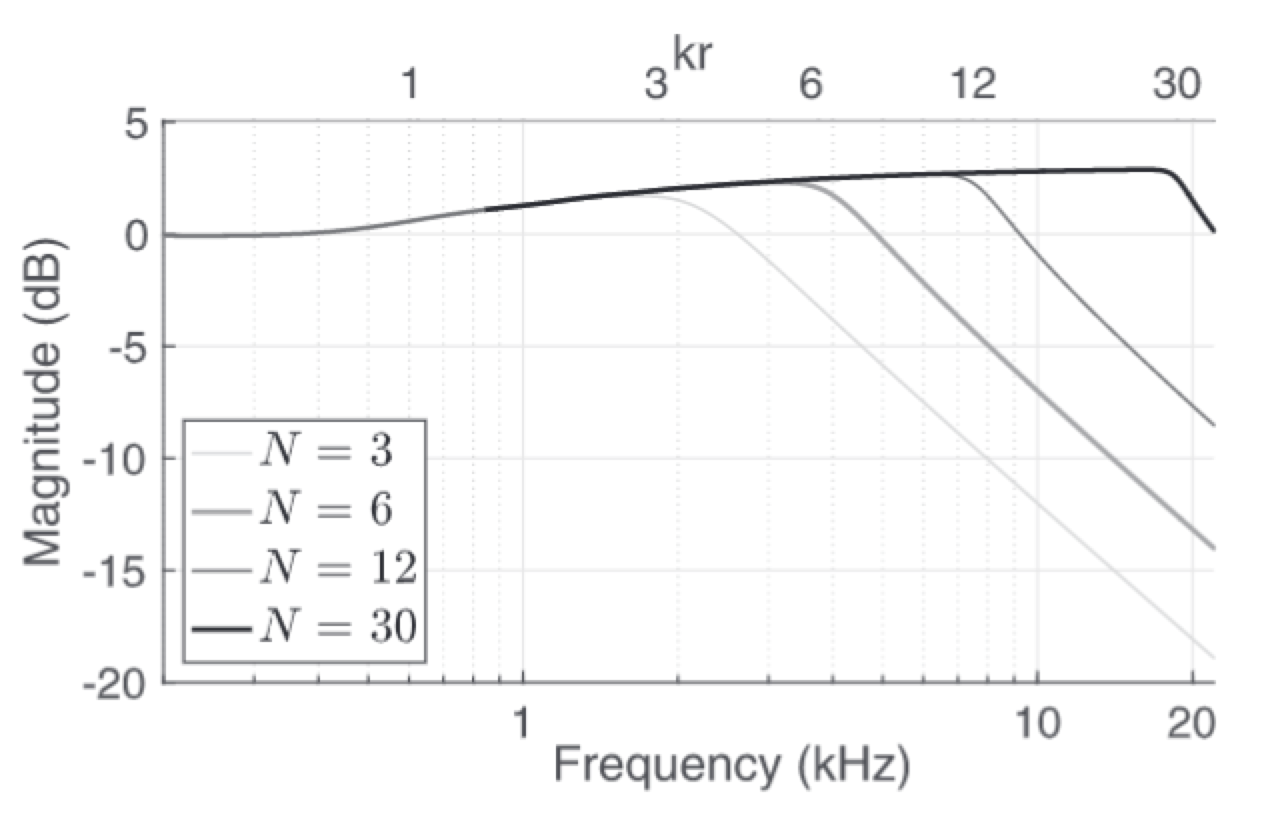
\includegraphics[clip,width=10cm]{./high_freq_rolloff.png}
    \caption{球面調和展開次数$N$と剛球上の音圧(式\ref{rigid_sphere_pressure_avg})の関係(\cite{Ben-Hur2017-gm}のFig.2より引用)}
    \label{high_freq_rolloff}
\end{figure}

\cite{Sheaffer2014-bo}ではこの高域での減衰を補正するためのフィルタが提案されている.
具体的には,低い展開次数$N$によって生成されたバイノーラル信号を補正するためのフィルタは以下のように与えられる.
$$
    \left.H(k)\right|_{N \rightarrow N_{h}}=\frac{\overline{p(k r)}_{N_{h}}}{p(k r)_{N}}
$$

\subsection{High-Frequency Time-Aligned Binaural Decoding
    (TA)\cite{Schorkhuber2018-ql,Zaunschirm2018-mn}}
\cite{Zaunschirm2018-mn}で示されているように,音場の高周波成分のエネルギーは球面調和展開したときの高次の展開係数に含まれている.その様子を図\ref{high_order_energy}に示す.
図\ref{high_order_energy}はある頭部伝達関数データセットを球面調和展開したときの展開次数ごとの正規化エネルギーをプロットしており,低次の展開係数では高周波成分のエネルギーを含みきれておらず,高域のエネルギーを十分に再現するには展開次数を30まで上げる必要があることがわかる.

\begin{figure}[htbp]
    \centering
    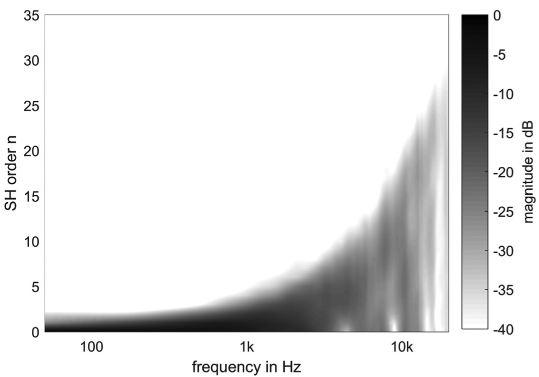
\includegraphics[clip,width=10cm]{./high_order_energy.png}
    \caption{ある頭部伝達関数データセットを球面調和展開したときの展開次数ごとの正規化エネルギーをプロットしたグラフ(\cite{Zaunschirm2018-mn}のFig.1より引用)}
    \label{high_order_energy}
\end{figure}

二重理論(duplex theory)によれば,ヒトが両耳間時間差(ITD)をほとんど低域でのみ音源定位の手がかりとして用いている\cite{roginska2017immersive}.
そこで\citeauthor{Zaunschirm2018-mn}\cite{Zaunschirm2018-mn}は高域での各周波数の位相を均一化し,
必要な展開次数を削減する手法を提案した.
位相均一化処理は以下のように定式化される.

$$
    h_{l, r}\left(\Omega_{p}, \omega\right)=h^{l, r}\left(\Omega_{p}, \omega\right) A_{p}^{l, r}(\omega)
$$

オールパスフィルタ$A_{p}^{l, r}(\omega)$の周波数特性は
$$
    A_{p}^{l, r}(\omega)=\left\{\begin{array}{ll}
        1                                                    & \text { for } \omega<\omega_{c}      \\
        e^{-i\left(\omega-\omega_{c}\right) \tau_{p}^{l, r}} & \text { for } \omega \geq \omega_{c}
    \end{array}\right.
$$

$\omega_c=2\pi f_c$はカットオフ角周波数,$\tau_{p}^{l, r}$は半径$r_H$の頭部の中心に対する点$p$(耳の位置)での信号の位相差である.

$$
    \tau_{p}^{r}=\cos \left(\theta_{p}\right) \sin \left(\phi_{p}\right) r_{H} c^{-1}, \quad \tau_{p}^{l}=-\tau_{p}^{r}
$$

図\ref{high_order_energy_improved}にTAC適応後の頭部伝達関数の展開次数ごとのエネルギー分布を示す.
図\ref{high_order_energy}と比較すると,高域でのエネルギーが低次元の展開次数に集中しており,展開次数を15ほど取ればTAC適応後の頭部伝達関数の高域のエネルギーを再現できることがわかる.

\begin{figure}[H]
    \centering
    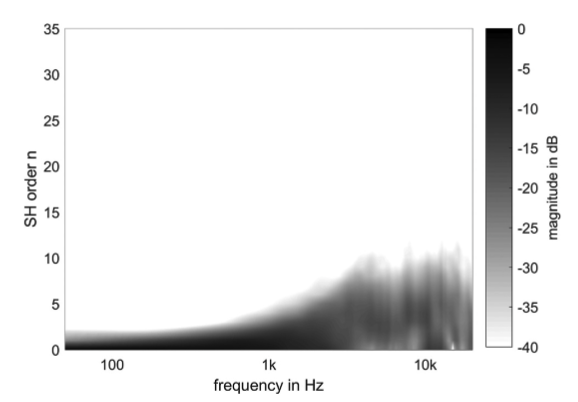
\includegraphics[clip,width=10cm]{./high_order_energy_improved.png}
    \caption{カットオフ周波数1.5kHzでTACを適応した頭部伝達関数データセットに対する展開次数ごとの正規化エネルギーをプロットしたグラフ(\cite{Zaunschirm2018-mn}のFig.4より引用)}
    \label{high_order_energy_improved}
\end{figure}
\cite{Schorkhuber2018-ql}によれば,カットオフ周波数は2kHzほどあれば主観的にも十分な結果が得られる.

\subsection{Diffuse-field Covariance-Constrained Binaural Renderer (TAC) \cite{Zaunschirm2018-mn}}

前節で提案されたTAに加え,\citeauthor{Zaunschirm2018-mn}\cite{Zaunschirm2018-mn}は音場の拡散性を考慮し,
両耳の頭部伝達関数の共分散行列を用いて最適なバイノーラル変換行列を算出する手法を提案している.
以下,\cite{Zaunschirm2018-mn}で提案された手法の概略を述べる.

遠距離場から周波数$\omega$, 角度$\Omega$から到来する原音場での音源を$s(\omega, \Omega)$とし,
頭部伝達関数を$\boldsymbol{h}(\omega, \Omega)=\left[h^{l}(\Omega, \omega), h^{r}(\Omega, \omega)\right]^{\top}$とすると,両耳での信号は

$$
    x(\omega)=\left[x^{l}(\omega), x^{r}(\omega)\right]^{\top}=\int_{S} s(\omega, \Omega) \mathbf{h(\omega, \Omega)} d \Omega
$$

対して,球面調和展開次数を$N_A$とすると,展開係数ベクトルは

$$
    \boldsymbol{a}(\omega)=\int_{S} s(\omega, \Omega) \boldsymbol{y}_{N_{A}}(\Omega) \mathrm{d} \Omega
$$

$$
    \boldsymbol{y}_{N_{A}}(\Omega)=\left[Y_{0}^{0}(\Omega), \ldots, Y_{n}^{m}(\Omega), \ldots, Y_{N_{A}}^{N_{A}}(\Omega)\right]^{\top}
$$

と書け,バイノーラル変換行列を$\mathbf{B_{N_A}}^H(\omega)$とするとバイノーラル再現信号は$\hat{\boldsymbol{x}}(\omega)=\boldsymbol{B}_{N_{\mathrm{A}}}^{\mathrm{H}}(\omega) \boldsymbol{a}(\omega)$と表すことができる.
原音場での両耳への入力信号$\boldsymbol{x}(\omega)$と$\hat{\boldsymbol{x}}(\omega)$の差を最小化するようなバイノーラル変換行列$\boldsymbol{B}_{N_{\mathrm{A}}}^{LS}$を求める最適化問題は以下のように定式化できる.

$$
    \boldsymbol{B}_{N_{A}}^{L S}(\omega)=\underset{\boldsymbol{B}_{N_{A}}(\omega)}{\arg \min } \int_{S}\left\|\boldsymbol{B}_{N_{A}}^{\mathrm{H}}(\omega) \boldsymbol{y}_{N_{A}}(\Omega)-\boldsymbol{h}(\omega, \Omega)\right\|_{\mathrm{F}}^{2} \mathrm{d} \Omega
$$

これを離散化すれば

\begin{equation}
    \label{least_square}
    \boldsymbol{B}_{N_{A}}^{L S}(\omega)=\underset{\boldsymbol{B}_{N_{A}}(\omega)}{\arg \min }\left\|\left(\boldsymbol{B}_{N_{A}}^{\mathrm{H}}(\omega) \boldsymbol{Y}_{N_{A}, P}-\boldsymbol{H}(\omega)\right) \boldsymbol{W}^{1 / 2}\right\|_{\mathrm{F}}^{2}
\end{equation}
where
$$
    \begin{array}{l}
        \boldsymbol{H}(\omega)=\left[\boldsymbol{h}_{1}(\omega), \ldots, \boldsymbol{h}_{p}(\omega), \ldots, \boldsymbol{h}_{P}(\omega)\right] \\
        \boldsymbol{h}_{p}(\omega)=\left[h^{l}\left(\Omega_{p}, \omega\right), h^{r}\left(\Omega_{p}, \omega\right)\right]^{\mathrm{T}}        \\
        \boldsymbol{Y}_{N_{A}, P}=\left[\boldsymbol{y}_{1}, \ldots, \boldsymbol{y}_{p}, \ldots, \boldsymbol{y}_{P}\right]                      \\
        \boldsymbol{y}_{p}=\left[Y_{0}^{0}\left(\Omega_{p}\right), \ldots, Y_{n}^{m}\left(\Omega_{p}\right), \ldots, Y_{N_{A}}^{N_{A}}\left(\Omega_{p}\right)\right]^{\mathrm{T}}
    \end{array}
$$
が得られる.$\mathbf{W}$は積分をガウス・ルジャンドル積分を用いて和に変換する際に用いる対角重み係数行列である.

ところで,頭部伝達関数の両耳に関する共分散行列は以下のように書ける.

$$
    \boldsymbol{R}_{H}= \int_{S} \boldsymbol{h}(\boldsymbol{\Omega}) \boldsymbol{h}^{\mathrm{H}}(\Omega) d \Omega = \begin{pmatrix}
        \int_{S} h^l(\boldsymbol{\Omega})^2 d \Omega                       & \int_{S} h^r(\boldsymbol{\Omega}) h^l(\boldsymbol{\Omega})d \Omega \\
        \int_{S} h^l(\boldsymbol{\Omega}) h^r(\boldsymbol{\Omega})d \Omega & \int_{S} h^2(\boldsymbol{\Omega})^2 d \Omega                       \\
    \end{pmatrix}
$$

これを離散化すれば,共分散行列は以下のように計算できる.

$$
    \boldsymbol{R}_{H} \cong \boldsymbol{H} \boldsymbol{W} \boldsymbol{H}^{\mathrm{H}}=\left[\begin{array}{cc}
            r^{l l}(\omega) & r^{l r}(\omega) \\
            r^{r l}(\omega) & r^{r r}(\omega)
        \end{array}\right]
$$

前節のTA処理を施した頭部伝達関数行列を$\mathbf{H}^\prime$とし,式\ref{least_square}において$\mathbf{H}$の代わりに$\mathbf{H}^\prime$を用いることを考える.
さらにバイノーラル変換行列が作る共分散行列行列が,頭部伝達関数が作る共分散行列と一致するという制約を加えるとバイノーラル変換行列は

\begin{equation}
    \label{least_square_tac}
    \begin{array}{l}
        \boldsymbol{B}_{N_{A}}^{T A C}=\underset{B_{N_{A}}}{\arg \min }\left\|\left(\boldsymbol{B}_{N_{A}}^{\mathrm{H}} \boldsymbol{Y}_{N_{A}, P}-\boldsymbol{H^\prime}\right) \boldsymbol{W}^{1 / 2}\right\|_{\mathrm{F}}^{2} \\
        \text { subject to } \boldsymbol{B}_{N_{A}}^{\mathrm{H}} \boldsymbol{R}_{Y} \boldsymbol{B}_{N_{A}}=\boldsymbol{R}_{H}
    \end{array}
\end{equation}

の解として得られる.式\ref{least_square_tac}の解の導出は煩雑であるため詳細は省くが,興味のある読者は\cite{Zaunschirm2018-mn}のSec.IIIを参照されたい.


\bibliographystyle{plainnat}
\bibliography{refs}

\end{document}